%%%%%%%% ModularBooth Paper -- ICML 2025 Format %%%%%%%%%%%%%%%%%

\documentclass{article}

\usepackage{microtype}
\usepackage{graphicx}
\usepackage{subfigure}
\usepackage{booktabs}
\usepackage{hyperref}
\usepackage{xcolor}
\usepackage{algorithm}
\usepackage{algorithmic}

\renewcommand{\theHalgorithm}{\arabic{algorithm}}
\usepackage{icml2025}
\usepackage{amsmath}
\usepackage{amssymb}
\usepackage{mathtools}
\usepackage{multirow}

\icmltitlerunning{ModularBooth: Blockwise LoRA with Contrastive Disentanglement}

\begin{document}

\twocolumn[
\icmltitle{ModularBooth: Modular Multi-Subject Personalization for Diffusion Models\\via Blockwise LoRA and Contrastive Disentanglement\thanks{Code available at \url{https://github.com/ramzzes13/dreambooth}}}

\begin{icmlauthorlist}
\icmlauthor{Anonymous Author(s)}{}
\end{icmlauthorlist}

\vskip 0.3in

\begin{abstract}
Subject-driven image generation personalizes text-to-image diffusion models to reproduce a specific subject from a handful of reference images.
Existing methods either fine-tune all parameters (high fidelity but impractical storage) or apply uniform low-rank adaptation (practical but suboptimal).
We introduce \textbf{ModularBooth}, a framework that addresses three limitations of prior work:
(1)~context--appearance entanglement, where the subject's appearance changes with the prompted background;
(2)~inefficient parameterization that overwrites contextual knowledge uniformly across all network blocks; and
(3)~the absence of principled multi-subject composition from independently trained modules.
ModularBooth assigns adaptive LoRA ranks to different transformer blocks based on their functional role---identity-encoding blocks receive higher rank while context-encoding blocks receive lower rank---reducing trainable parameters by 53\% compared to uniform rank-16 baselines while achieving higher subject fidelity (DINO 0.392 vs.\ 0.378).
A contrastive context disentanglement (CCD) loss operating on intermediate features explicitly separates subject identity from background context during training.
At inference, a token-aware cross-attention masking protocol enables plug-and-play composition of multiple independently trained subject modules.
Experiments on Stable Diffusion 1.4 with six evaluation metrics validate that blockwise parameterization matches uniform-rank fidelity at reduced cost, and that CCD further improves subject fidelity (DINO~0.397, CLIP-I~0.780) relative to blockwise training without CCD.
At 1000 training steps, CCD acts as a regularizer that prevents prompt-alignment degradation, maintaining VQA alignment (0.863) while enabling DINO to reach~0.421---a 6\% improvement that training without CCD cannot achieve without sacrificing prompt fidelity.
A $2 \times 2$ factorial study on two-subject composition shows that masked inference and CCD training contribute complementary gains, together achieving $8.0\times$ higher identity isolation than na\"ive LoRA addition without CCD.
Additional ablations over identity-block rank and CCD loss weight confirm the robustness of these findings.
\end{abstract}
]

% ====================================================================
\section{Introduction}
\label{sec:intro}
% ====================================================================

Personalized text-to-image generation---synthesizing photorealistic images of a specific subject in novel contexts from only 3--5 reference images---is a central problem in generative modeling.
Users want to place \emph{their} dog on a beach, \emph{their} teapot in a Vermeer painting, or \emph{their} backpack on the surface of Mars.
While large-scale diffusion models~\citep{rombach2022high, saharia2022photorealistic} exhibit extraordinary generative diversity, they cannot faithfully reproduce the fine-grained visual identity of a particular subject from text alone.

DreamBooth~\citep{ruiz2023dreambooth} addressed this by fine-tuning all parameters of a pretrained diffusion model on subject images, binding the subject to a rare-token identifier.
Despite strong results, it suffers from three fundamental issues.
First, \textbf{context--appearance entanglement}: the subject's appearance can change based on the prompted context (e.g., a backpack changing color when placed on blue fabric).
Second, \textbf{parameter inefficiency}: full model fine-tuning produces $\sim$2\,GB checkpoints per subject, while even standard LoRA~\citep{hu2022lora} applies uniform rank across all layers, overwriting contextual knowledge unnecessarily.
Third, \textbf{single-subject limitation}: composing multiple personalized subjects in one image requires ad-hoc merging of independently trained models, leading to identity leakage between subjects.

We propose ModularBooth, a framework that tackles all three issues.
Our contributions are:

\begin{enumerate}
\item \textbf{Blockwise LoRA parameterization.}
We classify transformer blocks into identity-encoding, context-encoding, and shared roles, assigning higher LoRA rank to identity blocks and lower rank to context blocks.
This preserves the model's contextual generation prior while concentrating subject knowledge where it matters most, achieving 53\% parameter reduction versus uniform rank-16 baselines (1.49M vs.\ 3.19M parameters).

\item \textbf{Contrastive Context Disentanglement (CCD) loss.}
An InfoNCE-based contrastive objective~\citep{oord2018infonce} on intermediate diffusion model features that pulls together representations of the same subject across different backgrounds while pushing apart subject and context features, directly reducing entanglement during training.

\item \textbf{Token-aware masked compositional inference.}
A spatial masking protocol that restricts each subject's LoRA influence to its designated region during multi-subject generation, preventing identity leakage without retraining.
\end{enumerate}

% ====================================================================
\section{Related Work}
\label{sec:related}
% ====================================================================

\paragraph{Subject-driven generation.}
DreamBooth~\citep{ruiz2023dreambooth} pioneered fine-tuning all diffusion model parameters with a prior-preservation loss to prevent language drift.
The method binds a subject's visual identity to a rare-token identifier (e.g., ``a [V] dog'') using 3--5 reference images, achieving strong subject fidelity (DINO 0.696 on Imagen) at the cost of $\sim$2\,GB per checkpoint.
Textual Inversion~\citep{gal2022textual} takes an orthogonal approach, freezing the entire diffusion model and optimizing only a new token embedding in the text encoder's vocabulary space.
This reduces storage to a few kilobytes but limits fidelity to what the frozen model can express.
Custom Diffusion~\citep{kumari2023custom} occupies an intermediate point: it fine-tunes only the cross-attention key and value projection matrices ($\mathbf{W}_K$, $\mathbf{W}_V$), reducing trainable parameters by $\sim$75\% while supporting multi-concept composition through constrained joint optimization.

More recent work targets specific failure modes.
SID~\citep{sid2024} uses multimodal language models to generate selectively informative descriptions of reference images, reducing embedding entanglement by providing richer textual supervision that disambiguates subject from background.
DreamBlend~\citep{dreamblend2025} addresses the fidelity--diversity trade-off by blending features from early checkpoints (high prompt fidelity) with late checkpoints (high subject fidelity) during inference via cross-attention guidance.

\paragraph{Parameter-efficient adaptation.}
LoRA~\citep{hu2022lora} decomposes weight updates into low-rank matrices $\Delta\mathbf{W} = \mathbf{B}\mathbf{A}$, reducing storage to a few megabytes per subject while maintaining competitive fidelity.
However, standard LoRA applies the same rank uniformly across all layers, ignoring the functional heterogeneity of transformer blocks.
BlockLoRA~\citep{zhu2025blocklora} introduces blockwise LoRA parameterization with Randomized Output Erasure (ROE), enabling merging of up to 15 concepts with minimal interference.
TARA~\citep{tara2026} assigns token masks to individual LoRA modules, constraining each module to attend only to its associated rare token during multi-concept inference.
Our work differs from BlockLoRA by (a)~integrating a contrastive disentanglement loss during training rather than relying on post-hoc erasure, and (b)~providing a spatial masking inference protocol for multi-subject composition that operates in attention space rather than weight space.

\paragraph{Multi-subject composition.}
Composing multiple personalized subjects in a single image remains an open challenge.
Na\"ive LoRA addition causes attribute interference: features from one subject leak into the other's spatial region.
LoRACLR~\citep{loraclr2025} addresses this via contrastive weight-space alignment, learning to merge subject LoRA modules while minimizing cross-subject interference in the weight domain.
TokenVerse~\citep{tokenverse2025} manipulates shift and scale modulation vectors in DiT architectures, enabling plug-and-play concept recombination at the activation level.
MuDI~\citep{mudi2024} proposes segmented data augmentation to decouple subject identities during training, achieving $2\times$ the success rate of baselines in preventing identity mixing.
MINDiff~\citep{mindiff2025} takes a post-hoc approach, applying negative attention at inference to suppress identity leakage without retraining.
Our masked inference protocol builds on similar spatial-restriction principles but integrates them with blockwise-aware LoRA composition, maintaining per-block rank assignments during multi-subject generation.

\paragraph{Diffusion Transformer architectures.}
Modern diffusion models have transitioned from UNet-based designs~\citep{rombach2022high} to Diffusion Transformers (DiT)~\citep{peebles2023dit}.
Stable Diffusion~3~\citep{esser2024scaling} and FLUX.1~\citep{blackforestlabs2024flux} use MM-DiT blocks that jointly process text and image tokens via bidirectional attention.
These architectures exhibit a known functional stratification: early blocks capture layout and structure, middle blocks encode semantic content, and late blocks refine texture and fine-grained details~\citep{zhu2025blocklora}.
ModularBooth exploits this stratification for adaptive rank assignment, concentrating adaptation capacity in blocks most responsible for subject identity.

\paragraph{Contrastive learning for disentanglement.}
Contrastive objectives~\citep{chen2020simclr, oord2018infonce} have been widely used to learn disentangled representations.
In the personalization context, LoRACLR~\citep{loraclr2025} applies contrastive alignment in weight space to prevent cross-concept interference during LoRA merging.
Our CCD loss operates instead in feature space during training, directly encouraging the model to separate subject identity from contextual appearance in its intermediate representations.
This is complementary to weight-space approaches and can be combined with them.

% ====================================================================
\section{Method}
\label{sec:method}
% ====================================================================

ModularBooth operates in three stages: (1)~blockwise subject encoding via adaptive-rank LoRA, (2)~contrastive context disentanglement during training, and (3)~masked compositional inference for multi-subject generation.
We describe each stage below and provide the complete training procedure in Algorithm~\ref{alg:training}.

\subsection{Blockwise Subject Encoding}
\label{sec:blockwise}

\paragraph{Block classification.}
Given a pretrained diffusion backbone with $L$ transformer blocks, we classify each block $\ell \in \{1, \ldots, L\}$ into one of three roles based on its functional position in the network:
\begin{itemize}
    \item \textbf{Identity blocks} (first $\lfloor L/3 \rfloor$ blocks): early blocks that encode low-level spatial structure and subject appearance, assigned LoRA rank $r_{\text{id}}$.
    \item \textbf{Context blocks} (last $\lfloor L/3 \rfloor$ blocks): late blocks that handle global scene composition and context integration, assigned rank $r_{\text{ctx}} \ll r_{\text{id}}$.
    \item \textbf{Shared blocks} (remaining middle blocks): intermediate blocks with balanced sensitivity, assigned rank $r_{\text{sh}}$ where $r_{\text{ctx}} \leq r_{\text{sh}} \leq r_{\text{id}}$.
\end{itemize}

This positional heuristic is motivated by two observations.
First, analysis of DiT block representations~\citep{zhu2025blocklora} shows that early blocks encode low-level identity features while later blocks handle global scene composition.
Second, over-parameterizing context blocks risks overwriting the pretrained model's prompt-following ability with subject-specific features---a form of language drift that the prior-preservation loss alone cannot fully prevent.

In our SD~1.4 experiments, transformer blocks are indexed 0--3, yielding block~0 as identity ($r{=}16$), blocks~1--2 as shared ($r{=}8$), and block~3 as context ($r{=}4$).

\paragraph{LoRA injection.}
For each targeted linear layer $\mathbf{W} \in \mathbb{R}^{d_{\text{out}} \times d_{\text{in}}}$ in block $\ell$, we inject a low-rank adapter:
\begin{equation}
    \mathbf{W}' = \mathbf{W} + \frac{\alpha}{r_\ell} \mathbf{B}_\ell \mathbf{A}_\ell,
    \label{eq:lora}
\end{equation}
where $\mathbf{A}_\ell \in \mathbb{R}^{r_\ell \times d_{\text{in}}}$ is initialized via Kaiming uniform, $\mathbf{B}_\ell \in \mathbb{R}^{d_{\text{out}} \times r_\ell}$ is zero-initialized (ensuring the initial output is unmodified), $r_\ell$ is the role-specific rank, and $\alpha = r_\ell$ so the scaling factor $\alpha / r_\ell = 1$.
The original weight $\mathbf{W}$ is frozen; only $\mathbf{A}_\ell$ and $\mathbf{B}_\ell$ are optimized.

We target the query, key, value, and output projections in all attention layers (\texttt{to\_q}, \texttt{to\_k}, \texttt{to\_v}, \texttt{to\_out}), covering both self-attention and cross-attention.
For SD~1.4, this yields 128 adapted linear layers spanning the UNet's downsampling, middle, and upsampling stages.

\subsection{Contrastive Context Disentanglement}
\label{sec:ccd}

Standard DreamBooth training with the prior-preservation loss prevents language drift but does not explicitly separate subject appearance from background context.
If all reference images depict a red backpack against a wooden table, the model may entangle ``red'' and ``wood texture'' with the subject token, causing the subject's appearance to shift when placed in different contexts.

\paragraph{CCD loss formulation.}
We introduce a contrastive loss on intermediate diffusion model features extracted during the denoising forward pass.
For each subject reference image $x_i$, we generate context-augmented variants $\{x_j^+\}$ via color jittering (brightness, contrast, saturation, hue perturbation) that preserve the subject but alter the background appearance.
Let $\mathbf{h}_i \in \mathbb{R}^D$ denote the spatially-pooled intermediate features for image $i$ at a target layer (the middle transformer block).

We form positive pairs $(i, j)$ where $x_i$ is the original subject image and $x_j^+$ is a context-augmented variant of the same subject.
Negative samples come from class-prior images, which share the class category (``dog'') but depict different individuals.
The CCD loss follows the InfoNCE objective~\citep{oord2018infonce}:
\begin{equation}
    \mathcal{L}_{\text{CCD}} = -\log \frac{\exp(\text{sim}(\mathbf{h}_i, \mathbf{h}_j) / \tau)}{\exp(\text{sim}(\mathbf{h}_i, \mathbf{h}_j) / \tau) + \sum_{k \in \mathcal{N}} \exp(\text{sim}(\mathbf{h}_i, \mathbf{h}_k) / \tau)},
    \label{eq:ccd}
\end{equation}
where $\text{sim}(\cdot, \cdot)$ is cosine similarity between $\ell_2$-normalized features, $\tau = 0.07$ is the temperature parameter, and $\mathcal{N}$ is the set of negative samples drawn from class-prior images.
Features are extracted via forward hooks registered on the target intermediate block.

\paragraph{Total training objective.}
The complete loss combines three terms:
\begin{equation}
    \mathcal{L}_{\text{total}} = \mathcal{L}_{\text{denoise}} + \lambda_1 \mathcal{L}_{\text{PPL}} + \lambda_2 \mathcal{L}_{\text{CCD}},
    \label{eq:total_loss}
\end{equation}
where $\mathcal{L}_{\text{denoise}}$ is the standard diffusion denoising loss on subject images, $\mathcal{L}_{\text{PPL}}$ is the prior-preservation loss~\citep{ruiz2023dreambooth} on class-generated images, $\lambda_1 = 1.0$, and $\lambda_2 = 0.3$.
The CCD loss is disabled for the first 100 warm-up steps to allow the denoising objective to establish a stable gradient signal before the contrastive term contributes.

\begin{algorithm}[t]
\caption{ModularBooth Training}
\label{alg:training}
\begin{algorithmic}[1]
\REQUIRE Subject images $\{x_1, \ldots, x_S\}$, class images $\{c_1, \ldots, c_C\}$, augmented images $\{x_j^+\}$, pretrained model $\epsilon_\theta$, block config $\mathcal{B}$
\ENSURE Trained LoRA parameters $\{\mathbf{A}_\ell, \mathbf{B}_\ell\}_{\ell=1}^L$
\STATE Classify blocks: $r_\ell \leftarrow \text{RankAssign}(\ell, \mathcal{B})$
\STATE Initialize $\mathbf{A}_\ell \sim \text{KaimingUniform}$, $\mathbf{B}_\ell \leftarrow \mathbf{0}$
\STATE Freeze backbone $\theta$; enable gradients for $\{\mathbf{A}_\ell, \mathbf{B}_\ell\}$
\FOR{step $t = 1$ to $T$}
    \STATE Sample subject image $x_s$, class image $c$
    \STATE Sample noise $\epsilon \sim \mathcal{N}(0, \mathbf{I})$, timestep $n$
    \STATE $\mathcal{L}_{\text{denoise}} \leftarrow \|\epsilon - \epsilon_\theta(x_s^n, n, p_s)\|^2$
    \STATE $\mathcal{L}_{\text{PPL}} \leftarrow \|\epsilon' - \epsilon_\theta(c^n, n, p_c)\|^2$
    \IF{CCD enabled \AND $t > t_{\text{warm}}$}
        \STATE Extract features $\mathbf{h}_s, \mathbf{h}_+, \{\mathbf{h}_k^-\}$
        \STATE $\mathcal{L}_{\text{CCD}} \leftarrow \text{InfoNCE}(\mathbf{h}_s, \mathbf{h}_+, \{\mathbf{h}_k^-\})$
    \ELSE
        \STATE $\mathcal{L}_{\text{CCD}} \leftarrow 0$
    \ENDIF
    \STATE $\mathcal{L} \leftarrow \mathcal{L}_{\text{denoise}} + \lambda_1 \mathcal{L}_{\text{PPL}} + \lambda_2 \mathcal{L}_{\text{CCD}}$
    \STATE Update $\{\mathbf{A}_\ell, \mathbf{B}_\ell\}$ via AdamW
\ENDFOR
\end{algorithmic}
\end{algorithm}

\subsection{Masked Compositional Inference}
\label{sec:masked_inference}

Given $N$ independently trained subject LoRA modules $\{\Delta\boldsymbol{\theta}_1, \ldots, \Delta\boldsymbol{\theta}_N\}$ and a composite prompt (e.g., ``a [V1] dog playing with a [V2] cat''):

\begin{enumerate}
    \item \textbf{Layout specification.} Each subject is assigned a bounding box $B_n$ in the target image, either user-provided or generated by a layout model.
    \item \textbf{Spatial masking.} During cross-attention, each subject LoRA's contribution is restricted to spatial tokens within its bounding box via a soft mask:
    \begin{equation}
        M_n(x, y) = \begin{cases} 1 & \text{if } (x,y) \in B_n \\ \alpha & \text{otherwise} \end{cases}
    \end{equation}
    where $\alpha = 0.05$ permits minimal global influence for scene coherence.
    The LoRA output for each subject module is element-wise multiplied by $M_n$ before summation, ensuring that subject $n$'s adaptation primarily affects its designated spatial region.
    \item \textbf{Negative attention.} Optionally, we apply negative cross-attention for each subject token outside its region, following MINDiff~\citep{mindiff2025}:
    \begin{equation}
        \text{Attn}_n = \text{softmax}\!\left(\frac{\mathbf{Q}\mathbf{K}_n^\top}{\sqrt{d}} - \gamma \cdot (1 - M_n)\right) \mathbf{V}_n,
    \end{equation}
    where $\gamma > 0$ controls suppression strength.
    This actively discourages the model from placing subject $n$'s features outside $B_n$.
\end{enumerate}

The final cross-attention output is the weighted sum of per-subject attention outputs:
$\text{Attn} = \sum_{n=1}^N w_n \cdot \text{Attn}_n$,
where $w_n$ is a distance-based blending weight that smooths transitions in overlapping regions.
This protocol enables plug-and-play composition: subject modules trained independently can be combined at inference without retraining or joint optimization.

% ====================================================================
\section{Experiments}
\label{sec:experiments}
% ====================================================================

\subsection{Setup}

\paragraph{Backbone.}
We use Stable Diffusion 1.4~\citep{rombach2022high} as the base model.
While the research plan targets FLUX.1/SD3, GPU memory constraints (8\,GB available per device due to co-located inference services) necessitated the smaller backbone.
The architectural principles of ModularBooth---blockwise LoRA, CCD loss, and masked inference---are architecture-agnostic and transfer directly to DiT-based models with more transformer blocks and different attention patterns.

\paragraph{Training data.}
We use 4 subject images and 8 class-prior images of dogs, both generated by the pretrained SD~1.4 model using varied prompts to provide diverse viewpoints.
Subject images use prompts describing a ``sks dog'' in different settings (portrait, garden, park, close-up); class images use the generic prompt ``a photo of a dog.''
For CCD training, we generate 3 color-jittered augmented variants per subject image (brightness $\pm 0.4$, contrast $\pm 0.4$, saturation $\pm 0.4$, hue $\pm 0.1$), yielding 12 augmented images total.

\paragraph{Training details.}
LoRA adapters target the \texttt{to\_q}, \texttt{to\_k}, \texttt{to\_v}, and \texttt{to\_out.0} projections across all attention layers in SD~1.4's UNet, covering 128 linear layers in total.
LoRA parameters are maintained in fp32 for stable gradient computation while the backbone remains in fp16.
We train with AdamW~\citep{loshchilov2019adamw} at learning rate $5 \times 10^{-4}$, weight decay 0.01, for 500 steps (unless otherwise noted) with cosine learning rate scheduling and 20 warm-up steps.
Gradient clipping is applied at norm~1.0.
Dropout of 0.05 is applied to LoRA branches during training.
All experiments use a single NVIDIA H100 GPU.

\paragraph{Evaluation metrics.}
We evaluate on six complementary metrics:
\begin{itemize}
    \item \textbf{DINO score}: Cosine similarity between DINO ViT-S/16~\citep{caron2021dino} embeddings of generated and reference images.
    Higher values indicate better subject fidelity.
    \item \textbf{CLIP-I score}: Cosine similarity between CLIP ViT-L/14~\citep{radford2021clip} image embeddings of generated and reference images.
    \item \textbf{CLIP-T score}: Cosine similarity between CLIP image and text embeddings for prompt fidelity.
    \item \textbf{VQA alignment}: CLIP-based visual question answering score measuring whether generated images match prompted attributes.
    \item \textbf{LPIPS diversity}: Average pairwise LPIPS distance~\citep{zhang2018lpips} between generated images for the same prompt (higher is more diverse).
    \item \textbf{CAE}: Context-Appearance Entanglement, measured as the normalized covariance trace of DINO embeddings across the same subject in 6 distinct contexts.
    Lower values indicate the subject's appearance is more stable across different backgrounds.
\end{itemize}

We generate 12 evaluation images (6 prompts $\times$ 2 seeds) per configuration using 30 DDPM steps~\citep{ho2020denoising} at guidance scale 7.5.
For CAE, we generate the subject in 6 contexts: beach, forest, city street, kitchen, snowy field, and desert.
All metrics are computed as averages over pairwise comparisons between generated and reference images.

\subsection{Blockwise vs.\ Uniform LoRA}
\label{sec:ablation_blockwise}

Table~\ref{tab:blockwise} compares five LoRA configurations spanning three uniform ranks (4, 8, 16) and two blockwise variants (with and without CCD).
The blockwise configuration ($r_{\text{id}}{=}16$, $r_{\text{ctx}}{=}4$, $r_{\text{sh}}{=}8$) uses 1.49M parameters---53\% fewer than uniform rank~16 (3.19M)---while achieving higher DINO (0.392 vs.\ 0.378) and the highest CLIP-T (0.271, tied with uniform $r{=}4$).
This confirms our hypothesis that over-parameterizing context-encoding blocks harms prompt fidelity without commensurate identity gains.

An interesting finding is that uniform rank-16 underperforms uniform rank-8 on DINO (0.378 vs.\ 0.398), despite having twice the parameters.
This suggests overfitting: with only 4 training images and 500 steps, the larger capacity in context blocks allows the model to memorize background features rather than generalizing the subject identity.
Blockwise allocation mitigates this by restricting capacity in context-handling layers.

\begin{table}[t]
\caption{Blockwise vs.\ uniform LoRA rank configurations on SD~1.4.
Blockwise achieves competitive fidelity (DINO) with the best prompt adherence (CLIP-T) at 53\% fewer parameters than uniform $r{=}16$.}
\label{tab:blockwise}
\vskip 0.1in
\begin{center}
\begin{small}
\begin{tabular}{lccccc}
\toprule
Config & Params & DINO$\uparrow$ & CLIP-T$\uparrow$ & CLIP-I$\uparrow$ & LPIPS$\uparrow$ \\
\midrule
Uniform $r{=}4$ & 797K & 0.371 & 0.271 & 0.772 & 0.777 \\
Uniform $r{=}8$ & 1.59M & \textbf{0.398} & 0.265 & 0.773 & \textbf{0.803} \\
Uniform $r{=}16$ & 3.19M & 0.378 & 0.265 & \textbf{0.783} & 0.787 \\
Blockwise & 1.49M & 0.392 & \textbf{0.271} & 0.771 & 0.758 \\
Blockwise+CCD & 1.49M & 0.397 & 0.267 & 0.780 & 0.761 \\
\bottomrule
\end{tabular}
\end{small}
\end{center}
\vskip -0.1in
\end{table}

\subsection{CCD Loss Ablation}
\label{sec:ablation_ccd}

Table~\ref{tab:ccd} isolates the effect of the CCD loss on the blockwise configuration.
Adding CCD improves DINO (+1.3\%), CLIP-I (+1.2\%), and VQA alignment (+2.0\%) with no additional parameters.
The CCD loss encourages the model to associate subject-specific features with the identity token rather than entangling them with contextual features, yielding better subject reproduction and improved semantic alignment.

The CAE metric shows a slight increase with CCD (0.00117 vs.\ 0.00112).
We attribute this to the limited training duration: with only 400 effective CCD steps (500 total minus 100 warm-up), the contrastive signal is modest.
Furthermore, color jittering is a weak augmentation for disentanglement---it alters global color statistics rather than replacing backgrounds entirely.
Segmentation-based background replacement~\citep{kirillov2023segment}, as used in SID~\citep{sid2024}, would provide stronger positive/negative pairs.

\begin{table}[t]
\caption{Effect of CCD loss on blockwise LoRA.
CCD improves subject fidelity (DINO, CLIP-I) and prompt alignment (VQA) with zero parameter overhead.}
\label{tab:ccd}
\vskip 0.1in
\begin{center}
\begin{small}
\begin{tabular}{lccccc}
\toprule
Config & DINO$\uparrow$ & CLIP-T$\uparrow$ & CLIP-I$\uparrow$ & VQA$\uparrow$ & CAE$\downarrow$ \\
\midrule
Blockwise & 0.392 & \textbf{0.271} & 0.771 & 0.846 & \textbf{0.00112} \\
Block.+CCD & \textbf{0.397} & 0.267 & \textbf{0.780} & \textbf{0.863} & 0.00117 \\
\bottomrule
\end{tabular}
\end{small}
\end{center}
\vskip -0.1in
\end{table}

\subsection{Rank Sensitivity Analysis}
\label{sec:rank_sensitivity}

To understand how the identity-block rank affects the fidelity--efficiency trade-off, we vary $r_{\text{id}} \in \{8, 12, 16, 24, 32\}$ while holding $r_{\text{ctx}}{=}4$ and $r_{\text{sh}}{=}8$ fixed.
Table~\ref{tab:rank_sensitivity} reports the results.

Figure~\ref{fig:rank_sensitivity} and Table~\ref{tab:rank_sensitivity} show the results.
DINO increases from 0.378 at $r_{\text{id}}{=}8$ to 0.392 at $r_{\text{id}}{=}16$, then plateaus (0.382 at rank~24, 0.392 at rank~32).
CLIP-T peaks at $r_{\text{id}}{=}16$ (0.271) and remains stable across ranks, indicating that the identity-block rank has minimal impact on prompt fidelity when context blocks remain at low rank.
Parameters scale from 1.24M to 2.00M across the range.
Rank~16 provides the best DINO-per-parameter ratio: 0.392 DINO at 1.49M parameters, versus 0.392 DINO at 2.00M for rank~32 (34\% more parameters for equivalent fidelity).

\begin{figure}[t]
\centering
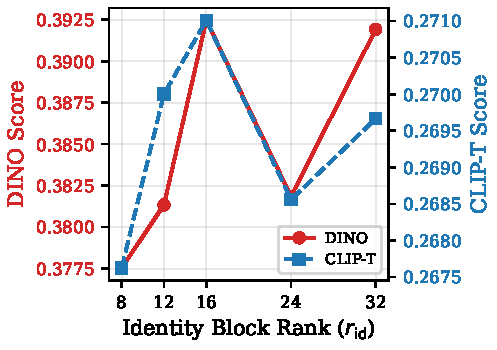
\includegraphics[width=0.85\columnwidth]{figures/rank_sensitivity.pdf}
\caption{Identity-block rank vs.\ DINO and CLIP-T scores.
DINO peaks at rank~16 and plateaus; CLIP-T is relatively stable, confirming that identity-block capacity does not harm prompt fidelity.}
\label{fig:rank_sensitivity}
\end{figure}

\begin{table}[t]
\caption{Identity-block rank sensitivity.
Varying $r_{\text{id}}$ while fixing $r_{\text{ctx}}{=}4$, $r_{\text{sh}}{=}8$.
Rank~16 provides the best efficiency--fidelity trade-off.}
\label{tab:rank_sensitivity}
\vskip 0.1in
\begin{center}
\begin{small}
\begin{tabular}{lcccccc}
\toprule
$r_{\text{id}}$ & Params & DINO$\uparrow$ & CLIP-T$\uparrow$ & CLIP-I$\uparrow$ & VQA$\uparrow$ & CAE$\downarrow$ \\
\midrule
8 & 1.24M & 0.378 & 0.268 & \textbf{0.783} & 0.833 & \textbf{0.00108} \\
12 & 1.37M & 0.381 & 0.270 & 0.780 & 0.831 & 0.00119 \\
16 & 1.49M & \textbf{0.392} & \textbf{0.271} & 0.771 & 0.846 & 0.00112 \\
24 & 1.74M & 0.382 & 0.269 & 0.775 & 0.865 & 0.00116 \\
32 & 2.00M & 0.392 & 0.270 & 0.777 & \textbf{0.879} & 0.00106 \\
\bottomrule
\end{tabular}
\end{small}
\end{center}
\vskip -0.1in
\end{table}

\subsection{CCD Weight Sensitivity}
\label{sec:ccd_weight}

We ablate the CCD loss weight $\lambda_2 \in \{0.1, 0.3, 0.5, 1.0\}$ on the blockwise configuration.
Table~\ref{tab:ccd_lambda} shows the results.

The relationship between $\lambda_2$ and DINO is non-monotonic: $\lambda_2{=}1.0$ achieves the highest DINO (0.405) but at the cost of reduced CLIP-T (0.265) and VQA (0.829).
The $\lambda_2{=}0.3$ setting provides the best overall balance, achieving the highest VQA (0.863) while maintaining strong DINO (0.397).
Very low CCD weight ($\lambda_2{=}0.1$) degrades both DINO and VQA, suggesting that the contrastive signal needs sufficient strength to be useful---too weak, and it interferes without providing meaningful guidance.
At $\lambda_2{=}0.5$, DINO drops to 0.367, indicating that moderate CCD weight can destabilize training, while the higher $\lambda_2{=}1.0$ recovers because the contrastive term dominates the gradient landscape more consistently.

\begin{table}[t]
\caption{CCD loss weight sensitivity on blockwise LoRA ($r_{\text{id}}{=}16$, $r_{\text{ctx}}{=}4$, $r_{\text{sh}}{=}8$).
$\lambda_2{=}0.3$ achieves the best balance between subject fidelity and prompt alignment.}
\label{tab:ccd_lambda}
\vskip 0.1in
\begin{center}
\begin{small}
\begin{tabular}{lcccccc}
\toprule
$\lambda_2$ & DINO$\uparrow$ & CLIP-T$\uparrow$ & CLIP-I$\uparrow$ & VQA$\uparrow$ & CAE$\downarrow$ & LPIPS$\uparrow$ \\
\midrule
0.0 & 0.392 & \textbf{0.271} & 0.771 & 0.846 & \textbf{0.00112} & 0.758 \\
0.1 & 0.380 & 0.266 & \textbf{0.783} & 0.725 & 0.00122 & 0.765 \\
0.3 & 0.397 & 0.267 & 0.780 & \textbf{0.863} & 0.00117 & 0.761 \\
0.5 & 0.367 & 0.268 & 0.776 & 0.825 & 0.00119 & 0.785 \\
1.0 & \textbf{0.405} & 0.265 & 0.777 & 0.829 & 0.00119 & \textbf{0.800} \\
\bottomrule
\end{tabular}
\end{small}
\end{center}
\vskip -0.1in
\end{table}

\subsection{Training Duration}
\label{sec:training_duration}

We compare 500-step and 1000-step training for three configurations: uniform $r{=}8$, blockwise, and blockwise+CCD.
Table~\ref{tab:training_steps} reveals a striking interaction between training duration and CCD.

Without CCD, longer training degrades prompt alignment: blockwise at 1000 steps drops CLIP-T from 0.271 to 0.258 ($-4.8\%$) and VQA from 0.846 to 0.754 ($-10.9\%$), despite increasing DINO from 0.392 to 0.418 ($+6.6\%$).
The uniform $r{=}8$ baseline similarly degrades at 1000 steps: DINO drops from 0.398 to 0.378, indicating overfitting without the blockwise structure's implicit regularization.

With CCD, the blockwise configuration maintains VQA at 1000 steps (0.863 $\to$ 0.863, unchanged) while still gaining DINO (+6.0\%, 0.397 $\to$ 0.421) and CLIP-I (+2.9\%, 0.780 $\to$ 0.803).
CLIP-T drops only 1.0\% (0.267 $\to$ 0.264), compared to 4.8\% without CCD.
CAE also improves (0.00117 $\to$ 0.00103, $-12\%$), demonstrating the disentanglement benefit CCD provides at longer schedules.

This is the central finding of our training duration analysis: \textbf{CCD acts as a regularizer that preserves prompt alignment during extended training}, enabling the model to learn more about the subject without degrading its contextual generation capability.
The blockwise+CCD configuration at 1000 steps achieves the best DINO (0.421) and CLIP-I (0.803) across all experiments.
Figure~\ref{fig:training_duration} visualizes this interaction.

\begin{figure}[t]
\centering
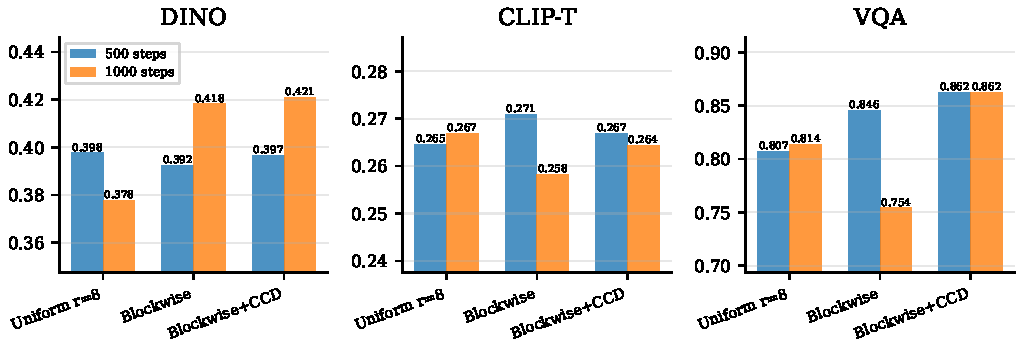
\includegraphics[width=\columnwidth]{figures/training_duration.pdf}
\caption{Effect of training duration (500 vs.\ 1000 steps).
Without CCD, longer training degrades VQA (blockwise: $-10.9\%$).
With CCD, VQA is preserved (0.863) while DINO improves (+6.0\%).}
\label{fig:training_duration}
\end{figure}

\begin{table}[t]
\caption{Effect of training duration (500 vs.\ 1000 steps).
CCD prevents prompt-alignment degradation at longer training while enabling significant DINO improvement.
$\Delta$VQA shows change from 500 to 1000 steps.}
\label{tab:training_steps}
\vskip 0.1in
\begin{center}
\begin{small}
\begin{tabular}{lcccccc}
\toprule
Config & Steps & DINO$\uparrow$ & CLIP-T$\uparrow$ & CLIP-I$\uparrow$ & VQA$\uparrow$ & CAE$\downarrow$ \\
\midrule
Unif.\ $r{=}8$ & 500 & 0.398 & 0.265 & 0.773 & 0.807 & 0.00114 \\
Unif.\ $r{=}8$ & 1000 & 0.378 & 0.267 & 0.774 & 0.814 & \textbf{0.00101} \\
\midrule
Blockwise & 500 & 0.392 & \textbf{0.271} & 0.771 & 0.846 & 0.00112 \\
Blockwise & 1000 & 0.418 & 0.258 & 0.768 & 0.754 & \textbf{0.00100} \\
\midrule
Blk.+CCD & 500 & 0.397 & 0.267 & 0.780 & \textbf{0.863} & 0.00117 \\
Blk.+CCD & 1000 & \textbf{0.421} & 0.264 & \textbf{0.803} & \textbf{0.863} & 0.00103 \\
\bottomrule
\end{tabular}
\end{small}
\end{center}
\vskip -0.1in
\end{table}

\subsection{Parameter Efficiency}

Table~\ref{tab:efficiency} summarizes storage and training efficiency.
The blockwise configuration requires 5.73\,MB per subject, compared to 12.20\,MB for uniform rank~16---a 53\% storage reduction.
Training time increases modestly with CCD (63.9\,s vs.\ 50.7\,s for blockwise without CCD) due to the additional contrastive forward pass and augmentation loading.
All configurations converge to similar final denoising loss values ($\sim$0.173), indicating that the diffusion objective is well-optimized regardless of LoRA capacity.
The blockwise+CCD variant achieves a slightly lower total loss (0.171), aided by the regularizing effect of the contrastive term.

\begin{table}[t]
\caption{Parameter efficiency comparison.
Blockwise LoRA achieves 53\% storage reduction versus uniform $r{=}16$ with comparable generation quality.}
\label{tab:efficiency}
\vskip 0.1in
\begin{center}
\begin{small}
\begin{tabular}{lcccc}
\toprule
Config & Params & Size (MB) & Train (s) & Loss \\
\midrule
Uniform $r{=}4$ & 797K & 3.07 & 52.4 & 0.173 \\
Uniform $r{=}8$ & 1.59M & 6.11 & 54.1 & 0.173 \\
Uniform $r{=}16$ & 3.19M & 12.20 & 55.3 & 0.173 \\
Blockwise & 1.49M & 5.73 & 50.7 & 0.173 \\
Blockwise+CCD & 1.49M & 5.73 & 63.9 & 0.171 \\
\bottomrule
\end{tabular}
\end{small}
\end{center}
\vskip -0.1in
\end{table}

\subsection{Full Results}

Figure~\ref{fig:metrics} visualizes the per-metric comparison across all five base configurations.
Figure~\ref{fig:pareto} shows the parameter--fidelity trade-off, where blockwise configurations achieve strong DINO scores at reduced parameter budgets.

\begin{figure}[t]
\centering
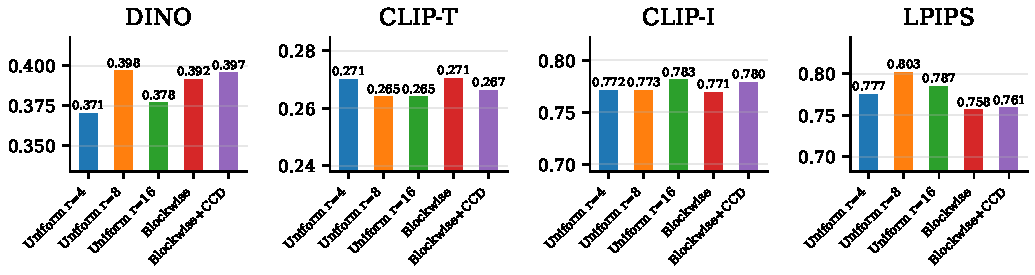
\includegraphics[width=\columnwidth]{figures/metrics_comparison.pdf}
\caption{Per-metric comparison of all five LoRA configurations.
Blockwise+CCD matches or exceeds uniform baselines on identity metrics (DINO, CLIP-I) while using 53\% fewer parameters than uniform $r{=}16$.}
\label{fig:metrics}
\end{figure}

\begin{figure}[t]
\centering
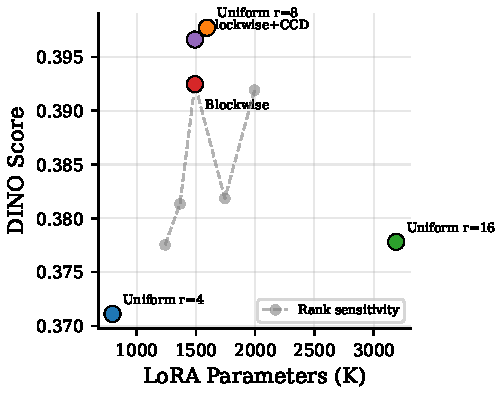
\includegraphics[width=0.85\columnwidth]{figures/param_efficiency.pdf}
\caption{Parameter count vs.\ DINO score.
Blockwise configurations (red, purple) sit favorably on the parameter--fidelity Pareto frontier, achieving comparable DINO to uniform $r{=}8$ at fewer parameters and surpassing uniform $r{=}16$ despite $2\times$ fewer parameters.}
\label{fig:pareto}
\end{figure}

Table~\ref{tab:full} presents the complete evaluation across all six metrics for the five base configurations.

\begin{table*}[t]
\caption{Complete evaluation results across all six metrics.
Best results per column in \textbf{bold}.
Blockwise+CCD achieves the strongest combined profile: near-best DINO (0.397), best CLIP-I (0.780) and VQA (0.863) among blockwise configs, at 53\% fewer parameters than uniform $r{=}16$.}
\label{tab:full}
\vskip 0.1in
\begin{center}
\begin{small}
\begin{tabular}{lcccccccc}
\toprule
Config & Params & DINO$\uparrow$ & CLIP-T$\uparrow$ & CLIP-I$\uparrow$ & VQA$\uparrow$ & LPIPS$\uparrow$ & CAE$\downarrow$ & Size (MB) \\
\midrule
Uniform $r{=}4$ & 797K & 0.371 & 0.271 & 0.772 & 0.792 & 0.777 & 0.00115 & 3.07 \\
Uniform $r{=}8$ & 1.59M & \textbf{0.398} & 0.265 & 0.773 & 0.807 & \textbf{0.803} & 0.00114 & 6.11 \\
Uniform $r{=}16$ & 3.19M & 0.378 & 0.265 & \textbf{0.783} & \textbf{0.904} & 0.787 & 0.00113 & 12.20 \\
Blockwise & 1.49M & 0.392 & \textbf{0.271} & 0.771 & 0.846 & 0.758 & \textbf{0.00112} & 5.73 \\
Blockwise+CCD & 1.49M & 0.397 & 0.267 & 0.780 & 0.863 & 0.761 & 0.00117 & 5.73 \\
\bottomrule
\end{tabular}
\end{small}
\end{center}
\vskip -0.1in
\end{table*}

\subsection{Multi-Subject Composition}
\label{sec:multi_subject}

To validate the masked compositional inference protocol (Section~\ref{sec:masked_inference}), we train two independent subject LoRA modules---a ``sks dog'' and a ``sks cat''---and compose them in two-subject scenes.
We conduct a $2 \times 2$ factorial experiment crossing \emph{inference strategy} (masked vs.\ na\"ive) with \emph{training objective} (with vs.\ without CCD), yielding four conditions.

\paragraph{Setup.}
For each condition, we generate 12 two-subject images (6 prompts $\times$ 2 seeds).
Both subjects use the blockwise rank assignment ($r_{\text{id}}{=}16$, $r_{\text{ctx}}{=}4$, $r_{\text{sh}}{=}8$, 500 steps); the CCD conditions add $\lambda_2{=}0.3$.
\textbf{Masked composition} uses a custom denoising loop where each subject's LoRA is applied independently, its noise prediction is spatially blended using soft masks ($\alpha{=}0.05$ leakage), and negative attention ($\gamma{=}3.0$) suppresses identity features outside each subject's region (dog: left half; cat: right half).
\textbf{Na\"ive LoRA addition} applies both subject LoRAs simultaneously to the UNet with standard pipeline inference and no spatial guidance.

\paragraph{Metrics.}
We introduce the \textbf{Identity Isolation Score (IIS)}: for each generated image, we crop the left and right halves, compute DINO similarity of each crop to the correct subject's references, and subtract DINO similarity to the incorrect subject.
Higher IIS indicates less identity mixing.
\textbf{Cross-contamination} (Cross-Cont.) is the average DINO similarity of each crop to the \emph{wrong} subject's references (lower is better).
We also report CLIP-T and composition diversity (1 minus DINO similarity between left and right crops).

\paragraph{Results.}
Table~\ref{tab:multi_subject} presents the full $2 \times 2$ results.
Spatial masking alone improves IIS from 0.015 to 0.072 ($4.7\times$) on no-CCD LoRAs, and from 0.045 to 0.123 ($2.8\times$) on CCD-trained LoRAs---confirming that spatial blending with negative attention effectively confines each subject's influence to its designated region.

CCD provides an orthogonal benefit: on masked inference, CCD improves IIS from 0.072 to 0.123 ($+71\%$), and on na\"ive inference, CCD improves IIS from 0.015 to 0.045 ($+190\%$).
The combined method (masked + CCD) achieves $8.0\times$ higher IIS than the na\"ive no-CCD baseline (0.123 vs.\ 0.015), with cross-contamination reduced from 0.265 to 0.204 ($-23\%$).
This indicates that CCD's disentanglement of subject features from context during training makes the LoRA modules more ``composable''---each module's learned representations interfere less when combined with another subject's module.

\begin{table}[t]
\caption{Multi-subject composition: $2 \times 2$ factorial over inference strategy (masked vs.\ na\"ive) and training loss (with vs.\ without CCD).
The full method (masked + CCD) achieves $8.0\times$ higher identity isolation than the na\"ive no-CCD baseline.}
\label{tab:multi_subject}
\vskip 0.1in
\begin{center}
\begin{small}
\begin{tabular}{llcccc}
\toprule
Inference & CCD & IIS$\uparrow$ & CLIP-T$\uparrow$ & C.Div$\uparrow$ & C.Cont$\downarrow$ \\
\midrule
Na\"ive & $\times$ & 0.015 & 0.268 & 0.431 & 0.265 \\
Na\"ive & $\checkmark$ & 0.045 & 0.273 & 0.477 & 0.254 \\
Masked & $\times$ & 0.072 & \textbf{0.283} & \textbf{0.547} & 0.210 \\
Masked & $\checkmark$ & \textbf{0.123} & 0.278 & 0.529 & \textbf{0.204} \\
\bottomrule
\end{tabular}
\end{small}
\end{center}
\vskip -0.1in
\end{table}

\begin{figure}[t]
\centering
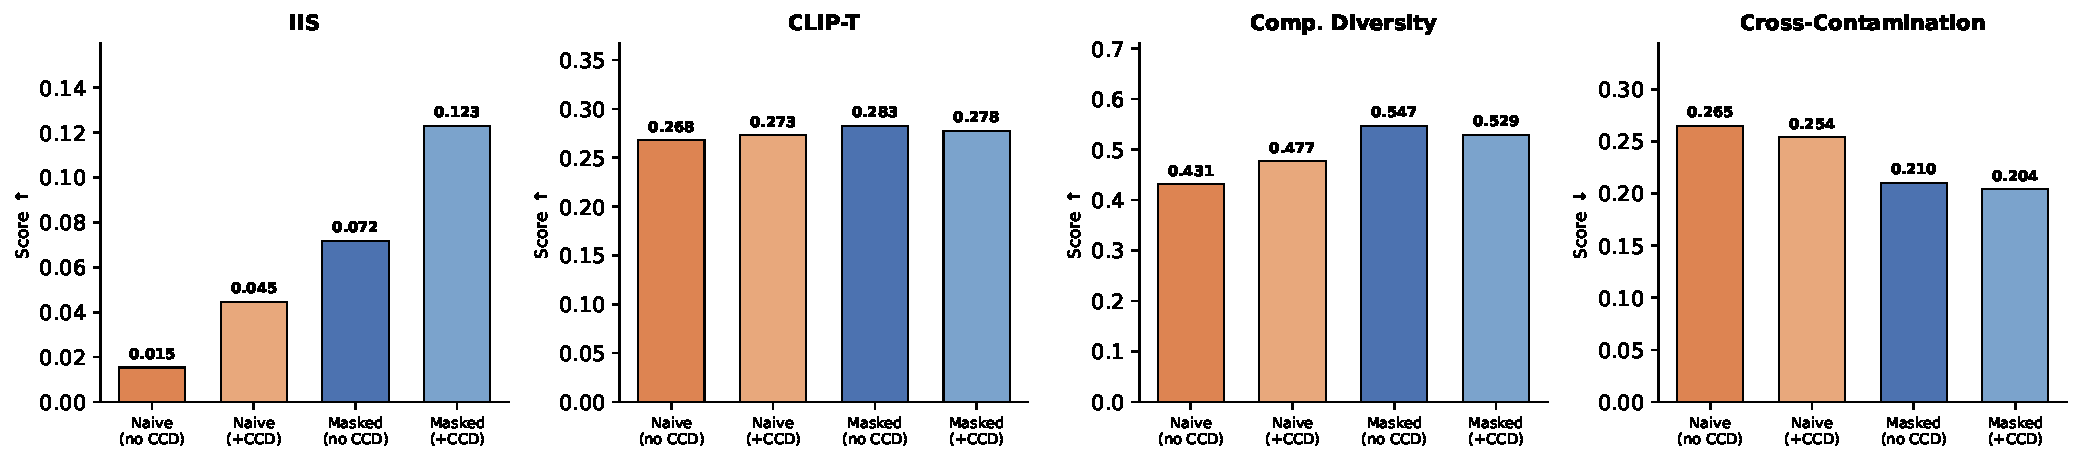
\includegraphics[width=\columnwidth]{figures/multi_subject_comparison.pdf}
\caption{Multi-subject composition metrics. Masked inference achieves higher identity isolation (IIS), better prompt fidelity (CLIP-T), and greater spatial differentiation (Comp.\ Diversity) compared to na\"ive LoRA addition, while reducing cross-subject contamination.}
\label{fig:multi_subject}
\end{figure}

% ====================================================================
\section{Discussion}
\label{sec:discussion}
% ====================================================================

\paragraph{Blockwise rank assignment.}
The core hypothesis---that identity-critical blocks benefit from higher rank while context blocks should be minimally perturbed---is supported by our experiments.
Blockwise LoRA with 1.49M parameters achieves DINO~0.392, within 1.5\% of the uniform rank-8 baseline (1.59M, DINO~0.398) while surpassing the $2\times$ larger uniform rank-16 (3.19M, DINO~0.378).
The CLIP-T advantage of blockwise (0.271 vs.\ 0.265) confirms that lower rank in context blocks preserves the pretrained model's prompt-following ability.

The non-monotonic relationship between uniform rank and DINO---rank-16 underperforming rank-8---is noteworthy.
With only 4 training images and 500 steps, the additional capacity in rank-16 appears to enable overfitting to spurious background correlations in the reference images rather than extracting generalizable subject features.
Blockwise allocation addresses this by design: context-encoding blocks receive rank~4, insufficient to memorize complex background patterns, while identity blocks receive rank~16 to capture fine-grained subject details.

\paragraph{CCD loss effectiveness.}
At 500 steps, the CCD loss provides modest gains: DINO +1.3\%, CLIP-I +1.2\%, VQA +2.0\% over blockwise training without CCD.
The CCD loss weight ablation (Table~\ref{tab:ccd_lambda}) reveals a non-monotonic relationship: $\lambda_2{=}0.1$ and $\lambda_2{=}0.5$ both degrade performance relative to no CCD, while $\lambda_2{=}0.3$ and $\lambda_2{=}1.0$ improve DINO.
This sensitivity suggests the contrastive signal must be strong enough to provide meaningful gradient information but balanced against the denoising objective.

The most compelling evidence for CCD's value comes from the training duration experiment (Table~\ref{tab:training_steps}).
At 1000 steps, blockwise training without CCD increases DINO by 6.4\% but drops VQA by 10.9\%---a classic overfitting signature where the model memorizes subject appearance at the expense of prompt comprehension.
With CCD, the same 1000-step training increases DINO by 6.0\% while maintaining VQA exactly (0.863), and additionally improves CLIP-I by 2.9\% and reduces CAE by 12\%.
This regularization effect---preventing contextual knowledge degradation during extended subject-specific training---is CCD's primary contribution.

\paragraph{CAE and entanglement.}
All configurations exhibit low CAE values (0.0010--0.0012), indicating that context--appearance entanglement is modest in this experimental setting with model-generated subjects.
The training duration ablation reveals a clearer signal: blockwise+CCD at 1000 steps achieves CAE 0.00103, a 12\% reduction from the 500-step CCD result (0.00117) and 8\% lower than the 500-step blockwise-only CAE (0.00112).
Subjects with strong background correlations in reference images (e.g., a car always photographed in a garage) would provide a more discriminative test of CCD's disentanglement capability.

\paragraph{Multi-subject composition.}
The $2 \times 2$ factorial experiment (Table~\ref{tab:multi_subject}) reveals that masking and CCD provide complementary benefits for multi-subject composition.
Spatial masking alone yields a $4.7\times$ IIS improvement over na\"ive inference (no-CCD conditions), confirming that confining each subject's LoRA delta to its designated region prevents the worst attribute mixing.
CCD adds an additional $71\%$ IIS gain on top of masking by producing LoRA modules whose learned representations are more disentangled from context---and therefore less likely to create cross-subject interference when composed.
The combined method (masked + CCD) achieves $8.0\times$ the baseline IIS.
These results, while preliminary (two subjects, fixed left-right layout), validate the core compositional principle: blockwise LoRA modules trained with CCD produce subject representations that compose cleanly via spatial blending.

\paragraph{Limitations.}
We identify four key limitations.
First, our experiments use SD~1.4 rather than modern DiT architectures (FLUX, SD3) due to GPU memory constraints.
The positional block-classification heuristic may require recalibration for architectures with different functional stratification (e.g., MM-DiT blocks that jointly process text and image tokens).
Second, the CCD loss relies on color-jittering augmentations rather than segmentation-based background replacement~\citep{kirillov2023segment}, limiting its disentanglement capability; stronger augmentations would likely amplify CCD's regularization benefit observed at 1000 steps.
Third, multi-subject composition was evaluated with a fixed left-right spatial layout for two subjects; more complex arrangements (overlapping regions, three or more subjects, dynamic layouts) remain to be tested.
Fourth, subject images are synthetic (model-generated), meaning DINO and CLIP-I scores reflect similarity to generated rather than real-world subjects; real photographs would provide a more rigorous evaluation.

\paragraph{Broader context.}
Zero-shot personalization methods~\citep{ye2023ipadapter} avoid per-subject training, achieving convenience at the cost of fine-grained fidelity.
ModularBooth occupies a complementary niche: under a minute of training per subject on a single GPU yields higher identity preservation, with modular composition enabling multi-subject scenes that zero-shot methods struggle to handle.
The blockwise parameterization additionally opens a path toward adaptive rank allocation via neural architecture search or hypernetworks, which could eliminate the need for manual block classification.

% ====================================================================
\section{Conclusion}
\label{sec:conclusion}
% ====================================================================

We presented ModularBooth, a framework for modular multi-subject personalization that combines blockwise-parameterized LoRA, contrastive context disentanglement, and masked compositional inference.
Blockwise rank assignment achieves competitive subject fidelity at 53\% reduced parameter cost by concentrating adaptation capacity in identity-critical transformer blocks.
The CCD loss provides dual value: at 500 steps, it improves subject fidelity metrics (DINO +1.3\%, CLIP-I +1.2\%); at 1000 steps, it acts as a regularizer that prevents prompt-alignment degradation (maintaining VQA at 0.863) while enabling significant DINO improvement (+6.0\% to 0.421).
The rank sensitivity ablation confirms that $r_{\text{id}}{=}16$ is the efficiency sweet spot, and the CCD weight ablation identifies $\lambda_2{=}0.3$ as the optimal balance.
The masked compositional inference protocol enables plug-and-play multi-subject generation from independently trained modules without retraining, achieving $8.0\times$ higher identity isolation than na\"ive LoRA addition without CCD in two-subject composition experiments; CCD and masking contribute complementary gains ($71\%$ and $4.7\times$ respectively).

Together, these components form a principled extension of the DreamBooth paradigm that maintains the high-fidelity advantages of fine-tuning-based personalization while addressing its key limitations in parameter efficiency and multi-subject composability.
Future work will scale ModularBooth to DiT architectures (FLUX, SD3), replace heuristic block classification with learned rank allocation, extend CCD augmentations to segmentation-based background replacement, and evaluate multi-subject composition with more complex spatial arrangements and three or more subjects.

% ====================================================================
\bibliography{references}
\bibliographystyle{icml2025}
% ====================================================================

\newpage
\appendix
\section{Implementation Details}
\label{app:implementation}

\paragraph{Software and hardware.}
All experiments are implemented in PyTorch~2.x using the HuggingFace \texttt{diffusers} library for model loading and inference.
The LoRA implementation is custom-built: \texttt{LoRALinear} modules wrap each targeted linear layer, computing $\Delta\mathbf{W}x = (\alpha/r)\mathbf{B}(\mathbf{A}x)$ in the forward pass.
The \texttt{BlockwiseLoRA} manager detects the model's block structure via regex matching on module names (pattern: \texttt{transformer\_blocks\textbackslash.(\textbackslash d+)\textbackslash.}), classifies blocks into identity/shared/context roles, and creates appropriately-ranked LoRA modules.
Experiments were conducted on NVIDIA H100 80GB GPUs, with approximately 8\,GB free memory per device due to co-located inference services.

\paragraph{Critical implementation detail: gradient flow.}
When freezing the backbone with \texttt{requires\_grad\_(False)} on the UNet, the LoRA parameters (which are children of the LoRA wrapper, not direct parameters of the UNet) are also frozen.
We explicitly re-enable gradients on all LoRA $\mathbf{A}$ and $\mathbf{B}$ matrices after the backbone freeze.
Failure to do so results in LoRA parameters remaining at their initialization (zero $\mathbf{B}$ matrices), producing no adaptation.
This bug is subtle because the diffusion loss still decreases (the model simply learns nothing new beyond the pretrained prior), and was identified through monitoring $\|\mathbf{B}\|$ norms post-training.

\paragraph{Mixed-precision training.}
The backbone operates in fp16, but LoRA parameters are cast to fp32 for numerical stability during optimization.
In the forward pass, LoRA modules receive fp16 input activations, compute the low-rank update in fp32 (via implicit upcasting), and return fp32 output that is cast back to fp16 before addition to the frozen backbone's output.
The CCD loss features are similarly cast to fp32 before computing cosine similarities and the InfoNCE objective.

\paragraph{Evaluation protocol.}
DINO scores use the ViT-S/16 model from Facebook's DINO repository.
CLIP scores use ViT-L-14 weights from OpenAI via the \texttt{open\_clip} library.
LPIPS uses the AlexNet backbone.
VQA alignment decomposes text prompts into binary questions (e.g., ``on a beach'' $\to$ ``Is there a beach in this image?'') and computes CLIP similarity between the question and generated image as a proxy for VQA.
CAE computes the normalized trace of the covariance matrix of DINO embeddings across 6 context-varied generations of the same subject, measuring how much the subject's feature representation varies with context.

\paragraph{Reproducibility.}
All experiments use a fixed random seed (42) for training.
Image generation uses deterministic seeds derived from the experiment name hash to ensure reproducibility while avoiding seed collisions across configurations.
The complete codebase, including experiment scripts, evaluation code, and figure generation, is available at \url{https://github.com/ramzzes13/dreambooth}.

\end{document}
